\documentclass[12pt,a4paper]{beamer}
\usetheme{Darmstadt}
\usepackage[latin1]{inputenc}

% Official title from the 283-Fahrplan, looks kinda stupid this way
\title[Open-GWAS]{Crowdsourcing Genome Wide Association Studies}%\\Freeing Genetic Data from Corporate Vaults}
% short title in [], long in {}
\date{28.12.2011}
\author{Bastian Greshake and Philipp Bayer}

\setbeamertemplate{navigation symbols}{} % get rid of unused symbols1

\begin{document}
\begin{frame}
\titlepage
\end{frame}

\begin{frame}{Overview}
\tableofcontents
\end{frame}

% The sections still have stupid names
\section{Introduction}
\subsection{Association studies}

\begin{frame}{What are GWAS?}
\begin{itemize}
\item Genome-wide Association Studies
\pause \item Link genetic variants (SNPs) to certain traits like Diabetes
\pause \item Compares groups carrying a certain SNP with groups without that SNP
\end{itemize}
\end{frame}

\begin{frame}{Single Nucleotide Polymorphism}
\begin{center}
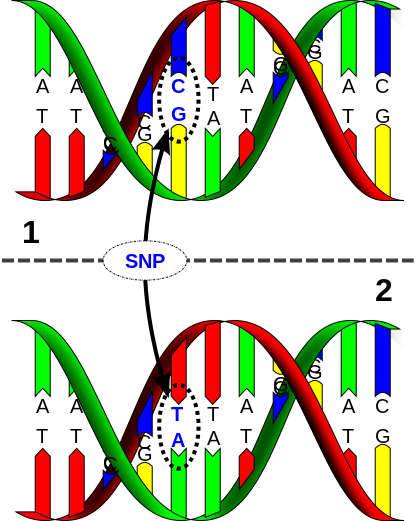
\includegraphics[scale=0.4]{SNP.png} \\
\begin{tiny}Source: http://en.wikipedia.org/wiki/File:Dna-SNP.svg\end{tiny}
\end{center}
\end{frame}

\begin{frame}{How do GWAS work?}
\begin{center}
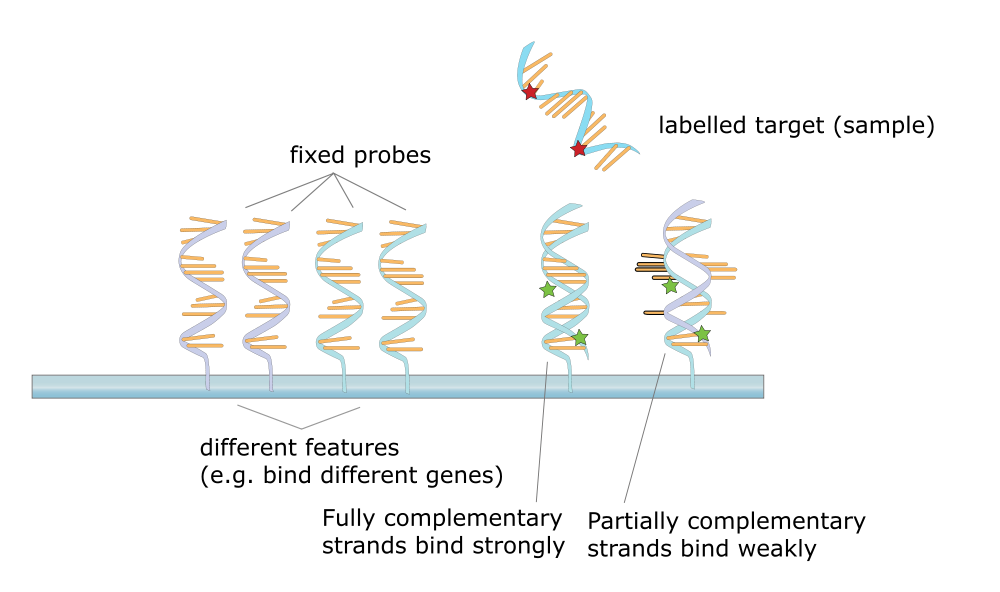
\includegraphics[scale=0.3]{microarray.png} \\
\begin{tiny}
Source: http://en.wikipedia.org/wiki/File:NA\_hybrid.svg
\end{tiny}
\end{center}
\end{frame}


\begin{frame}{Some GWAS-examples}
\begin{itemize}
\item Sladek \textit{et al.} (2007) identified four gene locations linked to heightened type 2 diabetes risk
\pause \item Kogan \textit{et al.} (2011) linked rs53576 (G:G) to pro-social behaviour
\pause \item The Wellcome Trust Case Control Consortium (2007) linked 24 locations to 7 major diseases 
\end{itemize}
\end{frame}

\begin{frame}{Personalised GWAS}
\begin{itemize}
\item 23andme: \$200 for a genotyping, 1.5 million SNPs + annotation
\pause \item Other companies (deCODEme...) similar price
\pause \item You get access to the raw data!
\end{itemize}
\end{frame}

\subsection{Open GWAS}
\begin{frame}{Why open GWAS?}
\begin{itemize}
\item DTC-Companies like 23andme keep their data locked up
\pause \item At least 100,000 datasets!
\pause \item No way for scientists to access the data
\pause \item Some customers uploaded their data to the net
\end{itemize}
\end{frame}

\section{Privacy}
\subsection{Privacy implications}
\begin{frame}{What can happen with open data?}
\begin{itemize}
\item Positive and negative consequences
\pause \item Possibly extremely bad consequences
\pause \item Up to you to decide whether you want to open your data
\end{itemize}
\end{frame}

\subsection{Consequences}
\begin{frame}{Positive consequences}
\begin{itemize}
\item More knowledge about yourself
\pause \item Cheap, open science
\pause \item Great data-source for citizen scientists
\end{itemize}
\end{frame}

\begin{frame}{Negative consequences}
\begin{itemize}
\item People know more about you than you'd like
\pause \item Your boss, your insurance company...
\pause \item Personal SNPs very similar to parents and relatives
\pause \item You could be carrying a deadly disease
\end{itemize}
\end{frame}

% maybe put this under positive consequences?


\begin{frame}{Open GWAS}
\begin{itemize}
\item No central repository for open genotypings!
\pause \item We've created openSNP.org
\pause \item open source repository for CC0-genotypings from 23andme, deCODEme and others
\pause \item Allows users to annotate with phenotypes (hair colour, nicotine dependence...)
\pause \item Scientists can download everything
\pause \item So far: 78 genotypings and 188 users % change before talk
\end{itemize}
\end{frame}

\section{Discussion}
% slight repition
\begin{frame}{Conclusions}
\begin{itemize}
\item Open GWAS are the future of personalised medicine
\pause \item It's in the hands of users to make or break the situation
\pause \item Chance to take science into our own hands %meh
\end{itemize}
\end{frame}

\subsection{Outlook}
\begin{frame}{Future of openSNP}
\begin{itemize}
\item We've won the PLoS/Mendeley Binary Battle
\pause \item Constantly improving the project
\pause \item Trying to get funds for free genotypings
\end{itemize}
\end{frame}

\begin{frame}{The end}
Thanks for listening. Any questions?
\end{frame}


\begin{frame}{References}
\begin{tiny}
Kogan, \textit{et al.} (2011): Thin-slicing study of the oxytocin receptor (OXTR) gene and the evaluation and expression of the prosocial disposition. Proceedings of the National Academy of Sciences\\
Sladek \textit{et al.} (2007): "A genome-wide association study identifies novel risk loci for type 2 diabetes". Nature 445 (7130): 881-5. \\
The Wellcome Trust Case Control Consortium  (2007): Genome-wide association study of 14,000 cases of seven common diseases and 3,000 shared controls. Nature 447: 661-678.\\
\end{tiny}
\end{frame}
\end{document}